\documentclass[a4paper,12pt,twoside,openright,titlepage]{book}

%Additional packages
\usepackage[utf8]{inputenc}
\usepackage[T1]{fontenc}
\usepackage[dutch,english]{babel}
\usepackage{syntonly}
\usepackage[official]{eurosym}

% Handle images
%\usepackage[graphicx]
\usepackage{graphicx}
\graphicspath{ {./images/}{./styles/} }
\usepackage{float}
\usepackage{wrapfig}

% Handle URLs
\usepackage{xurl}
\usepackage{hyperref}
\hypersetup{colorlinks=true, linkcolor=blue, citecolor=blue, filecolor=blue, urlcolor=blue, pdftitle=, pdfauthor=, pdfsubject=, pdfkeywords=}

% Tables and listings
\usepackage{multirow,tabularx}
\usepackage[table]{xcolor} % Table colors
\usepackage{scrextend}
\addtokomafont{labelinglabel}{\sffamily}
\usepackage{listings}
\usepackage{adjustbox}

% Turn on indexing
\usepackage{imakeidx}
\makeindex[intoc]

% Define colors
\usepackage{color}
\definecolor{ashgrey}{rgb}{0.7, 0.75, 0.71}


\usepackage{csquotes}

% Listing style
\lstset{
  backgroundcolor=\color{ashgrey}, % choose the background color; you must add \usepackage{color} or \usepackage{xcolor}; should come as last argument
  rulecolor=\color{black},         % if not set, the frame-color may be changed on line-breaks within not-black text (e.g. comments (green here))
  frame=single,	                   % adds a frame around the code
  basicstyle=\ttfamily,  % the size of the fonts that are used for the code
  extendedchars=true,    % lets you use non-ASCII characters; for 8-bits encodings only, does not work with UTF-8
  breakatwhitespace=true, % sets if automatic breaks should only happen at whitespace
  breaklines=true,        % sets automatic line breaking
  keepspaces=true,        % keeps spaces in text, useful for keeping indentation of code (possibly needs columns=flexible)
  columns=fullflexible,	  % Make sure no extra spaces are added.
  showstringspaces=false, % if true show spaces in strings adding particular underscores
  showspaces=false        % show spaces everywhere adding particular underscores; it overrides 'showstringspaces'
}



% Uncomment for production
% \syntaxonly

% Style
\pagestyle{headings}

% Define document
\author{D. Leeuw}
\title{Linux Basis Systeembeheer}
\date{\today\\v.0.4.0}

\begin{document}
\selectlanguage{dutch}

\maketitle

\copyright\ 2021-2023 Dennis Leeuw\\

\begin{figure}

\includegraphics[width=0.3\textwidth]{CC-BY-SA-NC.png}
\end{figure}

\bigskip

Dit werk is uitgegeven onder de Creative Commons BY-NC-SA Licentie en laat anderen toe het werk te kopi\"eren, distribueren, vertonen, op te voeren, en om afgeleid materiaal te maken, zolang de auteurs en uitgever worden vermeld als maker van het werk, het werk niet commercieel gebruikt wordt en afgeleide werken onder identieke voorwaarden worden verspreid.


%%%%%%%%%%%%%%%%%%%
%%% Introductie %%%
%%%%%%%%%%%%%%%%%%%

\frontmatter
\chapter{Over dit Document}
%Dit document behandeld Linux voor het middelbaar beroepsonderwijs in Nederland, maar kan breder ingezet worden, daar het gericht is op het behalen van het LPI Linux Essentials examen. De doelgroep is niveau 4 van het MBO, met enige kennis van computers.

\section*{Versienummering}
Het versienummer van elk document bestaat uit drie nummers gescheiden door een punt. Het eerste nummer is het major-versie nummer, het tweede nummer het minor-versienummer en de laatste is de nummering voor bug-fixes.\par
Om met de laatste te beginnen als er in het document slechts verbeteringen zijn aangebracht die te maken hebben met type-fouten, websites die niet meer beschikbaar zijn, of kleine foutjes in de opdrachten dan zal dit nummer opgehoogd worden. Als docent of student hoef je boek niet te vervangen. Het is wel handig om de wijzigingen bij te houden.\par
Als er flink is geschreven aan het document dan zal het minor-nummer opgehoogd worden, dit betekent dat er bijvoorbeeld plaatjes zijn vervangen of geplaatst/weggehaald, maar ook dat paragrafen zijn herschreven, verwijderd of toegevoegd, zonder dat de daadwerkelijk context is veranderd. Een nieuw cohort wordt aangeraden om met deze nieuwe versie te beginnen, bestaande cohorten kunnen doorwerken met het boek dat ze al hebben.\par
Als het major-nummer wijzigt dan betekent dat dat de inhoud van het boek substantieel is gewijzigd om bijvoorbeeld te voldoen aan een nieuw kwalificatiedossier voor het onderwijs of een nieuwe versie van Linux Essentials van de LPI. Een nieuw major-nummer betekent bijna altijd voor het onderwijs dat in het nieuwe schooljaar men met deze nieuwe versie aan de slag zou moeten gaan. Voorgaande versies van het document zullen nog tot het einde een schooljaar onderhouden worden, maar daarna niet meer.

\section*{Document ontwikkeling}
Het doel is door middel van open documentatie een document aan te bieden aan zowel studenten als docenten, zonder dat hier hoge kosten aan verbonden zijn en met de gedachte dat we samen meer weten dan alleen. Door samen te werken kunnen we meer bereiken.\par
Bijdragen aan dit document worden dan ook met alle liefde ontvangen. Let u er wel op dat materiaal dat u bijdraagt onder de CC BY-NC-SA licentie vrijgegeven mag worden, dus alleen origineel materiaal of materiaal dat al vrijgegeven is onder deze licentie.\par
De eerste versie is geschreven voor het ROC Horizon College.

%\begin{flushleft}
\begin{table}[h!]
\centering
\begin{tabularx}{\textwidth}{ |c|c|c|X| }
\hline
	Versienummer &
	Auteurs &
	Verspreiding &
	Wijzigingen\\
\hline
	0.1.0 &
	Dennis Leeuw &
	Wim Onrust &
	Initieel document\\
\hline
	0.2.0 &
	Dennis Leeuw &
	HEITO18IB-A &
	Toegevoegd: versienummering, de shell, begin van werken met bestanden\\
\hline
\end{tabularx}
\caption{Document wijzigingen}
\label{table:1}
\end{table}
\end{flushleft}



%%%%%%%%%%%%%%%%%
%%% De inhoud %%%
%%%%%%%%%%%%%%%%%
\tableofcontents

\mainmatter
%\chapter{Inleiding}
%Deze Linux cursus beoogt aan te sluiten bij het Linux Essentials examen van de LPI (Linux Professional Institute) en dient als voorbereiding op het MBO ICT Systems and Devices Expert examen. De cursus bestaat uit drie delen in het eerste deel installeren we CentOS als werkstation en leren we een grafische interface van het Linux systeem kennen. In het tweede deel werken we op de command line (CLI) en blijven we de CentOS installatie gebruiken. In deel 3 installeren we Debian en zullen we meer leren over Linux als server. De keuze om CentOS als werkstation te installeren en Debian als server is volledig willekeurig. Het doel is dat de studenten kennis maken met de rpm en dpkg package managers en leren dat het ene Linux systeem het andere niet is.

Alle Linux systemen zullen ge\"installeerd worden als virtuele machines op Virtual Box (\url{https://www.virtualbox.org/}). Door gebruik te maken van virtuele machines zijn we niet afhankelijk van de onderliggende hardware. De keuze voor VirtualBox heeft te maken met het feit dat dit product gratis te gebruiken is en beschikbaar is voor zowel Windows, Mac OS X als Linux.

Voor de CentOS machine is 15G vrije schijfruimte nodig en voor het Debian systeem 8G, wat een totaal aan 23G vrije schijfruimte vereist. Voor elke machine hebben we 2G RAM nodig, dus een totaal van 4G RAM moet vrij beschikbaar zijn.

%Management netwerk

%\chapter{Debian installatie}
%Selecteer de Grafische installatie interface in de Debian Installer Menu (\ref{DebInstallMenu}).

\begin{figure}[H]
	\centering
	\includegraphics[width=\linewidth]{debian_install_01.png}
	\caption{Debian Installer Menu}
	\label{DebInstallMenu}
\end{figure}

Selecteer daarna de Engelse taal. Dit is de taal die gebruikt wordt voor de installatie. De taal van het OS kiezen we later.

Bij Location kiezen we eerst other en daarna Europe en dan Netherlands. Voor de Locales laten we staan en\_US.UTF-8. Voor de keyboard houden we American English aan, tenzij je een specifiek toetsenbord hebt.

De volgende keuze die je moet maken is die voor een hostname, kortom hoe gaat je computer heten. Ik heb gekozen voor DNC01, wat staat voor Debian NextCloud eerste machine. De keuze voor het domein waarin de machine zit is lastig omdat we geen domein hebben. Het makkelijkst is om hier voorlopig localdomain in te vullen. We kunnen het later altijd nog wijzigen.

Nu moeten we een root wachtwoord kiezen, omdat we diensten gaan draaien op deze machine is het verstandig om een sterk wachtwoord te kiezen. Ook voor de gebruiker is dat een goed plan. Gebruik een password manager om een wachtwoord te generen of om je gekozen wachtwoorden erin op te slaan.

We houden de harddisk indeling simpel, dus kiezen we Guided als onze optie voor de harddisk indeling zoals aangegeven in \ref{DebDiskPart}.

\begin{figure}[H]
	\centering
	\includegraphics[width=\linewidth]{debian_install_partition.png}
	\caption{Debian Disk Partitioning}
	\label{DebDiskPart}
\end{figure}

We kiezen de enige harddisk die er is en kiezen voor All files in one partition. In het overzicht dat we te zien krijgen zien we dat er naast een bestandssysteem ook een swap-partitie aangemaakt is zoals weergeven in figuur \ref{DebDiskParts}.

\begin{figure}[H]
	\centering
	\includegraphics[width=\linewidth]{debian_install_partitioned.png}
	\caption{Debian Disk Overview}
	\label{DebDiskParts}
\end{figure}

Nadat we hebben gekozen voor Yes bij de vraag of we het zeker weten zal Debian beginnen met de installatie van het systeem. Na de installatie van het base system (een minimaal systeem), krijgen we de vraag of we nog meer software van andere CD's willen installeren. Dat willen we niet. Debian gaat nu opzoek naar updates en additionele software die ge\"installeerd kan worden. De repo's van Debian staan over de wereld verspreid, om geen data op te halen van bijvoorbeeld servers in de Verenigde Staten, maar alleen van servers in Nederland, zodat de belasting van het Internet alleen lokaal is, moeten we een keuze maken vanaf welke servers wij onze software willen ophalen. Kies Netherlands en deb.debian.org. We gebruiken geen proxy dus bij die vraag mag je continue geven.

Debian gaat nu de databases ophalen van alle software die er voor Debian beschikbaar is en gaat daarna meteen je systeem updaten met de laatst beschikbare versies. Afhankelijk van hoe nieuw de ISO was waarvan de hebt geboot kan dit even duren. Je kan af en toe een vraag krijgen van de installer, lees de tekst dan goed en bepaal of je het wel of niet wil wat er gevraagd wordt. Als de update klaar is krijg je de keuze om nog extra software te installeren (zie \ref{DebSoft}).

\begin{figure}[H]
	\centering
	\includegraphics[width=\linewidth]{debian_install_software.png}
	\caption{Debian Additional Software Choice}
	\label{DebSoft}
\end{figure}

We willen geen desktop en ook geen printserver, dus deze twee opties moeten we uit zetten. De standard system utilities willen we wel, dus die laten we aan staan.

Nadat Debian klaar is met de installatie kiezen we ervoor om GRUB te installeren in de master boot record, we selecteren /dev/sda en als alles klaar is rebooten we het systeem.

Login als root en installeer het sudo pakket. Voeg daarna jezelf als gebruiker toe aan de sudo groep:
\begin{lstlisting}[language=bash]
# usermod -a -G sudo dennis
\end{lstlisting}
Vervang \texttt{dennis} door je eigen gebruikersnaam die je aangemaakt het bij de installatie.

We loggen uit als root en loggen vanaf nu alleen nog in als gewone gebruiker.


% requires: BIOS knowledge, bootloader
% provides: /boot/, grub, kernel, modules
\chapter{Booting Linux en /boot/}
Nadat het BIOS klaar is met zijn taken wil deze een boot-loader laden. Vroeger was dit LiLo, de Linux Loader, maar tegenwoordig wordt GRUB, GRand Unified Bootloader, gebruikt. GRUB kan verschillende operating systems laden en kan dus gebruikt worden als universele bootloader om zowel Linux als Windows te starten. Zo kan je op \'e\'en machine Windows en Linux hebben staan en kan je door te herstarten kiezen welk OS je wil gebruiken.

De bootloader laadt de kernel, Linux, welke ervoor zorgt dat er tegen de hardware gesproken kan worden. De taken van de kernel zijn:
\begin{itemize}
\item het beheren van het fysieke geheugen en daarbij behorend het opdelen van het virtuele geheugen voor proces isolatie
\item zorgen dat zowel processen als hardware de resources krijgen waarom ze vragen (interrupts), als dat mag
\item het serialiseren van de taken die uitgevoerd moeten worden, ofwel proces management (schedulig)
\end{itemize}

Als de kernel zijn taken verder op de achtergrond kan uitvoeren kan proces nummer 1 gestart worden om het verdere bootproces af te maken, meestal eindigend in een grafische of een command line interface, waarna de gebruiker(s) aanzet zijn.

Als je een \texttt{ls} doet van de \texttt{/boot/} directory dan vinden we daarin de belangrijkste bestanden die nodig zijn om een Linux systeem op te kunnen starten.


\section{GRUB Configuratie}
De configuratie van GRUB staat in \texttt{/etc/} en in \texttt{/boot/grub/} (soms in \texttt{/boot/grub2/} of een ander versienummer). De GRUB bestanden in \texttt{/boot/} zijn gegenereerde bestanden en daar zou je nooit zelf wijzigingen in moeten aanbrengen. De wijzigingen worden aangebracht in \texttt{/etc/default/grub} en de snippets in \texttt{/etc/grub.d}. Een script \texttt{grub-mkconfig} maakt van dit geheel de configuratie in in \texttt{/boot/}.


\section{Kernel boot bestanden}
De kernel\index{kernel}, Linux, bestaat uit een modulaire kernel. Er is een stuk basis software die geladen wordt tijdens het opstarten en deze software kan uitgebreid worden met modules\index{modules}. Modules voegen extra functionaliteit toe, zoals bij voorbeeld netwerk-drivers. De reden dat er gekozen voor een modulair design is dat de basis kernel daardoor klein kan zijn en minder geheugen inneemt. Alleen de drivers of andere functionaliteit die echt nodig is wordt geladen.

De basis kernel ook bekend als \texttt{vmlinuz}\index{vmlinuz} kan gevonden worden in de \texttt{/boot/}\index{/boot/} directory, in het verleden werd de kernel in de \texttt{/} directory gezet en kan daar op sommige systemen nog gevonden worden. In de \texttt{/boot/} directory kan je ook bestanden vinden die beginnen met vmlinuz en waarna er een serienummer volgt, zo kunnen er meerdere versies van de kernel staan, waaruit eventueel via de bootloader gekozen kan worden.

Naast het bestand \texttt{vmlinuz} staan er nog een paar bestanden die bij de kernel horen:
\begin{description}
\item[config] is de configuratie van de kernel zoals deze gebruikt is tijdens het compilen van de kernel. Het beschrijft o.a. welke stukken van de kernel als module gebouwd moeten worden. Dit document is niet belangrijk voor het opstarten van het systeem.
\item[initrd.img] Ook de kernel heeft tijdens het opstarten modules nodig, denk daarbij aan de netwerk-drivers. De \texttt{initrd.img} bevat deze drivers en deze image wordt in RAM geladen zodat de modules snel beschikbaar zijn (ipv. dat ze van een trage harddisk moeten komen)
\item[System.map] bevat een overzicht van welke functies of variabelen zich op welke lokatie bevinden in de kernel. Dit bestand wordt gebruikt om lookups te doen als er een kernel oops of kernel panic zich voordoet.
\end{description}


% requires: 
% provides: modules, lsmod, modprobe
\chapter{Werken met modules}
De modules die bij de kernel horen kunnen gevonden worden in de directories onder \texttt{/lib/modules/}\index{/lib/modules/}. De modules die behoren bij de draaiende kernel kunnen gevonden worden via:
\begin{lstlisting}[language=bash]
$ ls /lib/modules/`uname -r`/kernel/
\end{lstlisting}

Modules kunnen on-the-fly geladen worden. Een overzicht van de reeds geladen modules kan verkregen worden met \index{lsmod}:
\begin{lstlisting}[language=bash]
$ lsmod
\end{lstlisting}

Om te zorgen dat onze kernel kan omgaan met het FAT bestandssysteem gaan we de fat-modules toevoegen aan de draaiende kernel\index{modprobe}. Dit mag natuurlijk alleen root doen.
\begin{lstlisting}[language=bash]
$ sudo modprobe fat
\end{lstlisting}
Bij geen error-melding is alles goed gegaan. Dit kunnen we controleren
\begin{lstlisting}[language=bash]
$ lsmod | grep fat
\end{lstlisting}
Na deze handeling zouden we bijvoorbeeld een USB-stick met een FAT bestandssysteem kunnen lezen.

Het verwijderen van een module is zo simpel als aan \texttt{modprobe} vertellen met de \texttt{-r} optie dat het een module moet verwijderen
\begin{lstlisting}[language=bash]
$ sudo modprobe -r fat
\end{lstlisting}



% requires: kill, begrip van boot proces
% provides: systemd, Unit-files, systemctl
\chapter{Werken met daemons}
In de Unix wereld zeggen we altijd 'Everything is a file and if it is not a file it is a process'.

Processen die op de achtergrond draaien heten daemons in de Unix-wereld. Ze zijn ook bekend als services, zeker in de Windows wereld. Daemons zijn dus processen waar je weinig van merkt en die rustig hun werk staan te doen. Deze processen draaien zonder dat ze input van de gebruiker nodig hebben.

Bekende daemons zijn bijvoorbeeld een web- of mailservers, maar het kan ook een printserver zijn.


\section{init en systemd}
Nadat de kernel in het geheugen geladen is zal deze gestart worden. De Linux kernel zorgt ervoor dat de beschikbare hardware klaar is voor gebruik en dat er processen gestart kunnen worden. Het eerste proces dat de kernel start is \texttt{systemd}\index{systemd}. Vroeger was dit \texttt{init}\index{init} en dat kan je op vele ander Unix-achtige besturingssystemen nog tegen komen, maar de meeste Linux distributies zijn over naar \texttt{systemd}.

\texttt{systemd} is het proces dat ervoor zorgt dat alle ander processen gestart worden. De \texttt{systemd} daemon heeft proces nummer 1. Het is de eerste daemon die start bij het opstarten van het systeem en de laatste die afgesloten wordt bij het afsluiten van het systeem.

Naast de \texttt{systemd} daemon die de moeder is van alle processen, zijn er ook commando's waarmee je (als root) daemons kunt starten, stoppen en herstarten. Het commando dat doorvoor beschikbaar is heet \texttt{systemctl}\index{systemctl}. Een standaard met de installatie meegekomen daemon in de systemd-timesyncd\index{timesyncd}\index{systemd!timesyncd} daemon. We gaan deze daemon gebruiken om een beetje vertrouwd te raken met \texttt{systemctl}.

\begin{lstlisting}[language=bash]
sudo systemctl status systemd-timesyncd
\end{lstlisting}

\begin{figure}[h]
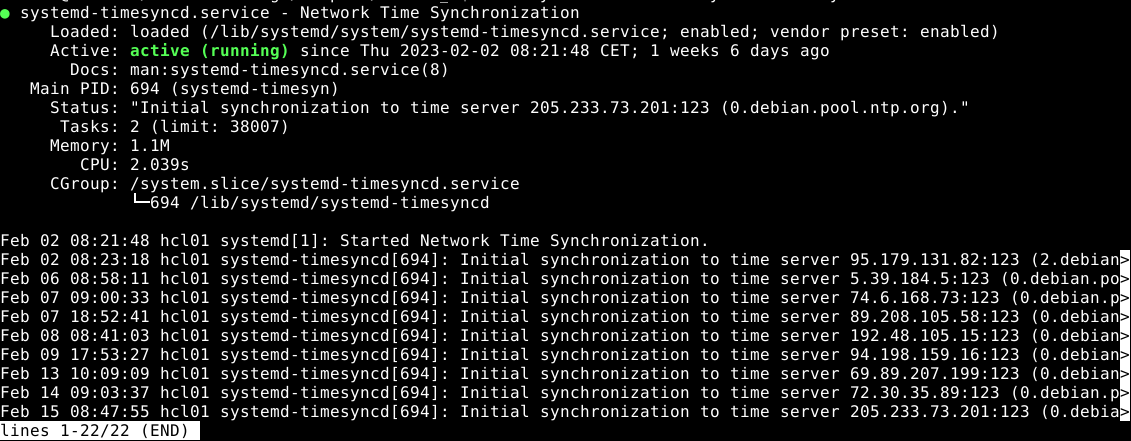
\includegraphics[width=8cm]{systemd-timesyncd-status}
\centering
	\caption{Status output van systemctl}
	\label{scrn:systemd-timesyncd-status}
\end{figure}

Als je net als in het voorbeeld (Figuur \ref{scrn:systemd-timesyncd-status}) een lijn hebt met END dan kan je gebruik maken van 'q' om weer op de command-prompt terecht te komen.

Door aan \texttt{systemctl} de commando's stop of start mee te geven kunnen we daemons op ons systeem stoppen en starten. De tijd synchronisatie daemon is op dit moment gestart, dus het eerste wat we kunnen doen is hem stoppen:

\begin{lstlisting}[language=bash]
sudo systemctl stop systemd-timesyncd
\end{lstlisting}

Met \texttt{systemctl status} kunnen nu de status van de daemon zien en dan zien we dat deze gestopt is. Het opnieuw opstarten doen we met start:

\begin{lstlisting}[language=bash]
sudo systemctl start systemd-timesyncd
\end{lstlisting}


\section{Unit files}
Om een service te starten of te stoppen gebruikt \texttt{systemd} bestanden waarin beschreven wordt hoe een service heet en welke commando's er nodig zijn om te starten en stoppen. Deze beschrijving van een service wordt binnen \texttt{systemd} een \textbf{unit} genoemd. Units kan je onder andere terug vinden in de \texttt{/etc/systemd/system} directory. Een voorbeeld van een unit-file in Debian 11 is de \texttt{syslog.service}. Deze ziet er zo uit:

\begin{lstlisting}[language=bash]
[Unit]
Description=System Logging Service
Requires=syslog.socket
Documentation=man:rsyslogd(8)
Documentation=man:rsyslog.conf(5)
Documentation=https://www.rsyslog.com/doc/

[Service]
Type=notify
ExecStart=/usr/sbin/rsyslogd -n -iNONE
StandardOutput=null
Restart=on-failure

# Increase the default a bit in order to allow many simultaneous
# files to be monitored, we might need a lot of fds.
LimitNOFILE=16384

[Install]
WantedBy=multi-user.target
Alias=syslog.service
\end{lstlisting}

Onder het kopje \textbf{Unit} vind je een beschrijving van de service en wat deze nodig heeft om te kunnen werken. Bij \textit{Requires} staat dat \texttt{syslog} een \texttt{syslog.socket} nodig heeft. Voor nu gaan we ervan uit dat het systeem dit oplost. Wij gaan verder naar de \textbf{Service} kop.

Bij \textit{ExecStart} staat het commando dat gebruikt moet worden op de service op te starten. Zoals je kan zien is er geen commando gegeven om de service te stoppen. Een Unix-achtig systeem heeft de \texttt{kill} functie om om te gaan met processen (zie Linux CLI documentatie). Deze kan gebruikt worden door \texttt{systemd} om processen te stoppen. De \textit{Type} met als waarde Notify zegt dat de daemon aan systemd laat weten wanneer het klaar is met opstarten. Dit heeft als voordeel dat als \texttt{systemd} dit signaal krijgt dat het door kan met andere zaken te doen en niet langer hoeft te wachten. Tot slot is er in deze sectie nog de \textit{Restart} optie die we willen behandelen. Het geeft niet aan wat we moeten doen bij een restart, maar wanneer we moeten restarten. In dit geval als \texttt{rsyslogd} crashed of elke andere willekeurig melding van een error geeft dan wordt het proces geherstart.

Alle Unit-files zijn platte tekst bestanden en kunnen dus met een willekeurige editor aangepast worden. Als je een bestand (service) hebt gewijzigd of toegevoegd moet je \texttt{systemctl} vertellen dat er iets nieuws is. Dat doe je met het volgende commando:
\begin{lstlisting}[language=bash]
$ sudo systemctl daemon-reload
\end{lstlisting}
Hierna kan je de nieuwe of aangepaste service stoppen, starten of herstarten met de gewijzigde settings.


\section{systemctl}
Na het opstarten van een systeem kan het soms nodig zijn met bestaande processen te stoppen of herstarten omdat er bijvoorbeeld een wijziging in de configuratie is gebeurd, of omdat bepaalde functionaliteit niet langer via deze machine aangeboden wordt. Het kan ook voorkomen dat nieuwe functionaliteit is toegevoegd en dat er een nieuw proces gestart moet worden. Het is dus van belang dat we \texttt{systemd} kunnen vertellen om deze acties uit te voeren. Het commando dat doorvoor beschikbaar is heet \texttt{systemctl}\index{systemctl}. \texttt{systemctl} kent een aantal standaard commando's die we kunnen meegeven. Voor een uitleg van de syntax van het commando verwijzen we naar de man-page. Wij behandelen hier alleen de belangrijkste commando's:
\begin{description}
	\item[start] Start een service
	\item[stop] Stop een service
	\item[restart] Stop een service en als dat klaar is start het weer
	\item[reload] Vraag een service om zijn configuratie opnieuw te laden, kan niet met alle daemons. Dit is niet de Unit-configuratie, maar de configuratie van de daemon zelf.
\end{description}

Om wat ervaring op te doen met \texttt{systemctl} gaan we wat oefenen met een daemon die standaard met de installatie is meegekomen en waar we wat mee kunnen spelen zonder dat het meteen destcructief is voor het systeem. De standaard met de installatie meegekomen daemon is de systemd-timesyncd\index{timesyncd}\index{systemd!timesyncd} daemon. We gaan deze daemon gebruiken om een beetje vertrouwd te raken met \texttt{systemctl}.

\begin{lstlisting}[language=bash]
sudo systemctl status systemd-timesyncd
\end{lstlisting}

\begin{figure}[h]
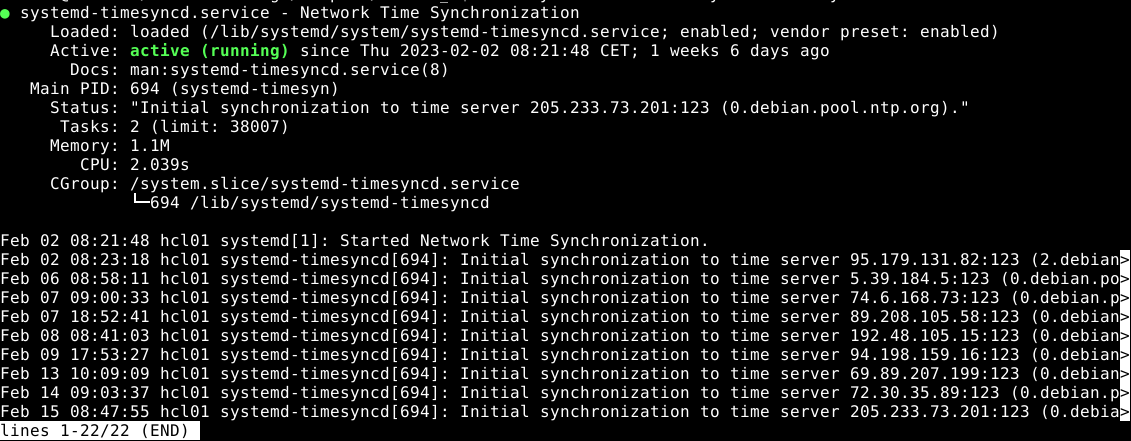
\includegraphics[width=8cm]{systemd-timesyncd-status}
\centering
	\caption{Status output van systemctl}
	\label{scrn:systemd-timesyncd-status}
\end{figure}

Als je net als in het voorbeeld (Figuur \ref{scrn:systemd-timesyncd-status}) een lijn hebt met END dan kan je gebruik maken van 'q' om weer op de command-prompt terecht te komen.

Door aan \texttt{systemctl} de commando's stop of start mee te geven kunnen we daemons op ons systeem stoppen en starten. De tijd synchronisatie daemon is op dit moment gestart, dus het eerste wat we kunnen doen is hem stoppen:

\begin{lstlisting}[language=bash]
sudo systemctl stop systemd-timesyncd
\end{lstlisting}

Met \texttt{systemctl status} kunnen nu de status van de daemon zien en dan zien we dat deze gestopt is. Het opnieuw opstarten doen we met start:

\begin{lstlisting}[language=bash]
sudo systemctl start systemd-timesyncd
\end{lstlisting}

Probeer nu zelf de herstart en reload functies uit. Wat neem je waar?



% requires: tail
% provides: syslog, rsyslog, systemd-journald, journalctl
\chapter{Logging}
Omdat daemons op de achtergrond draaien en geen direct contact met een gebruiker of met root hebben zullen ze op een andere manier moeten laten weten of het goed met ze gaat, wat ze aan het doen zijn en of de beheerder misschien moet ingrijpen omdat er iets fout gaat. Daemons laten ons weten wat er aan de hand is door hun berichten te loggen\index{logging}\index{loggen}. Loggen is het wegschrijven van de berichten naar een logbestand.

Linux systemen verzamelen alle log bestanden in een directory \texttt{/var/log}. Een daemon kan zelfstandig zijn eigen log wegschrijven naar een bestand, of de daemon kan gebruik maken van een log-server\index{log-server}. Het voordeel van een log-server is dat de daemon alleen de API van de log-server hoeft te kennen. Alle andere logica rond het loggen wordt afgehandel door de log-server. Voor meer informatie over de log-server zie de sectie over syslog (\ref{sec:syslog}).

Om direct te kunnen volgen wat er op een systeem gebeurt wordt veel het \texttt{tail} commando gebruikt. \texttt{tail} heeft een optie \texttt{-f} die follow betekent. Het blijft volgen welke nieuwe regels er aan een bestand worden toegevoegd. Een manier om bijvoorbeeld de \texttt{messages} log te blijven volgen is:
\begin{lstlisting}[language=bash]
$ sudo tail -f /var/log/messages
\end{lstlisting}

Omdat alle log-bestanden tekst bestanden zijn kan je ook bijvoorbeeld \texttt{grep} erop los laten en zo zoeken naar bepaalde patronen in de log-bestanden.


% provides: logrotate
\section{Log rotation}\label{sec:logrotate}
Als applicaties berichten loggen naar bestanden dan worden de log bestanden steeds langer en daarmee het systeem steeds trager. Dat is niet handig. Eens in de zoveel tijd moet een log-bestand dan ook geleegd worden, maar we willen de oude logs niet kwijt raken. Het proces dat ervoor zorgt dat logs op de juiste manier behandeld worden zodat ze niet te groot worden heet log rotate\index{log rotate}.

Er zijn verschillende manieren om het roteren van logs voor elkaar te krijgen. Natuurlijk kunnen we het handmatig doen. We moeten dan:
\begin{enumerate}
\item de daemon stoppen,
\item het log-bestand verplaatsen naar een andere naam (bijvoorbeeld, logbestand.backup),
\item een nieuw leeg log-bestand aanmaken met de juiste rechten,
\item de daemon opstarten.
\end{enumerate}
Dit is een hoop werk en tijdens het werk staat de daemon uit. Tevens is het elke keer dezelfde handeling, dus een prima klus om te automatiseren.

We kunnen een script schrijven dat dit doet en dat via cron laten draaien. Een andere optie is dat we een tool gebruiken die het voor ons regelt zoals bijvoorbeeld \texttt{logrotate}\index{logrotate}.


% provides: syslog, systemd-journald
\section{syslog}\label{sec:syslog}
Het proces dat op de achtergrond draait en dat verantwoordelijk is voor het schrijven van de verschillende logbestanden heet syslog\index{syslog}, een afkorting van system logging. Het gebruik van syslog heeft als groot voordeel dat niet elke software ontwikkelaar alle code hoeft te schrijven om logbestanden te schrijven, hij hoeft alleen maar te weten hoe hij data moet aanlever bij de syslog server. Voor de systeembeheerder is het makkelijk omdat hij niet elk programma hoeft te vertellen waar deze zijn meldingen weg moet schrijven, die hoeft alleen maar de syslog-server te beheren en het laatste voordeel is dat de output van syslog altijd dezelfde is, dus de logbestanden worden nog makkelijker leesbaar ook.

Vele Linux distributies gebruiken rsyslog\index{rsyslog} als hun syslog server. De belangrijkste logbestanden in de \texttt{/var/log} die beheerd worden door de syslog server zijn:
\begin{description}
\item[\texttt{messages}] Alle logs
\item[\texttt{mail} (SuSE) \texttt{maillog} (RedHat) of \texttt{mail.log} (Debian)] Mail logging
\item[\texttt{mail.info}] Mail info messages
\item[\texttt{mail.warn}] Mail warning messages
\item[\texttt{mail.err}] Mail error messages
\item[\texttt{daemon.log} (Debian)] Berichten van Daemons
\item[\texttt{auth.log} (Debian) of \texttt{secure} (RedHat)] Authenticatie gerelateerde berichten
\end{description}

\input{src/rsyslog}
% requires: logrotate systemd-journald
\section{journalctl}\label{sec:journalctl}
\texttt{systemd}\index{systemd} is het eerste proces (daemon) dat opgestart wordt op een Linux systeem. Het is daarmee de moeder van alle processen. Als er een daemon opgestart moet worden dan wordt dat gedaan via \texttt{systemd}. \texttt{systemd} is dus de plek waar ook in de gaten gehouden kan worden wat er opgestart is en wat niet en daarmee kan \texttt{systemd} een bijzondere inkijk geven in de status van een systeem. Om meer inzicht te krijgen in wat \texttt{systemd} allemaal voorbij heeft zien komen is er een tool met de naam \texttt{journalctl}\index{journalctl}.

Het opstarten van \texttt{journalctl} zonder enige opties of argumenten laat zien wat \texttt{systemd} heeft verzameld sinds het opstarten van het systeem, of sinds de laatste logrotate.

Om alleen de berichten te zien van een specifiek proces kunnen we het volgende commando gebruiken:
\begin{lstlisting}[language=bash]
$ sudo journalctl -f -u systemd-journald
\end{lstlisting}
De \texttt{-f} optie doet hetzelfde als bij \texttt{tail}, het zegt dat de log gevolgd (follow) moet worden. Met \texttt{-u} geef je op welke 'unit' er gemonitord moet worden.



% requires:
% provides: ps, netstat, ss
\chapter{Monitoring services}
In de sectie over \texttt{journalctl} hebben we gezien hoe we informatie over een proces kunnen opvragen. We kunnen zien of een daemon gestart of gestopt is. Daemons zijn processen die op de achtergrond draaien en die allerlei taken kunnen uitvoeren. Zo is \texttt{cron} een daemon, maar een daemon kan ook een mail-server of web-server zijn. Deze laatste twee luisteren op het netwerk naar inkomende verbindingen. De mail-server doet dat voor inkomende mail op poort 25 en de web-server op poort 80. Het is handig als we kunnen zien welke processen er draaien en wat ze aan het doen zijn. Dit hoofdstuk beschrijft enkele commando's die we daarvoor kunnen gebruiken.

\section{Proces monitoring}
In het document 'Linux CLI' hebben we \texttt{ps}\index{ps} behandeld. Met \texttt{ps} kan je zien welke processen er draaien op een systeem. In deze sectie gaan we \texttt{ps} met andere opties gebruiken dan we eerder hebben gedaan. De Linux variant van \texttt{ps} kent de mogelijkheid om ook opties te gebruiken zonder gebruik van het min teken voor de optie, dit is de zogenaamde BSD-style:
\begin{lstlisting}[language=bash]
$ ps aux
\end{lstlisting}
doet bijna hetzelfde als \texttt{ps -ef}. De output ziet er ook bijna hetzelfde uit:
\begin{lstlisting}[language=bash]
$ ps aux
USER         PID %CPU %MEM    VSZ   RSS TTY      STAT START   TIME COMMAND
root           1  0.0  0.0 167316 11924 ?        Ss   Feb02   0:48 /sbin/init
root           2  0.0  0.0      0     0 ?        S    Feb02   0:00 [kthreadd]
root           3  0.0  0.0      0     0 ?        I<   Feb02   0:00 [rcu_gp]
root           4  0.0  0.0      0     0 ?        I<   Feb02   0:00 [rcu_par_gp]
root           9  0.0  0.0      0     0 ?        I<   Feb02   0:00 [mm_percpu_wq]
root          10  0.0  0.0      0     0 ?        S    Feb02   0:00 [rcu_tasks_rude_]
root          11  0.0  0.0      0     0 ?        S    Feb02   0:00 [rcu_tasks_trace]
root          12  0.0  0.0      0     0 ?        S    Feb02   1:25 [ksoftirqd/0]
root          13  0.0  0.0      0     0 ?        I    Feb02   6:07 [rcu_sched]
root          14  0.0  0.0      0     0 ?        S    Feb02   0:03 [migration/0]
root          16  0.0  0.0      0     0 ?        S    Feb02   0:00 [cpuhp/0]
root          17  0.0  0.0      0     0 ?        S    Feb02   0:00 [cpuhp/1]
root          18  0.0  0.0      0     0 ?        S    Feb02   0:03 [migration/1]
root          19  0.0  0.0      0     0 ?        S    Feb02   0:10 [ksoftirqd/1]
\end{lstlisting}
De extra informatie is voornamelijk de extra data over het gebruik van de CPU en van het geheugen (MEM). Deze informatie kennen we ook uit de \texttt{top} applicatie. Ook dit commando is behandeld in de 'Linux CLI' handleiding.


\section{Daemons en netwerken}
Veel daemons worden gebruikt om diensten aan het netwerk aan te bieden. Om een dienst aan te kunnen bieden moet een daemon luisteren op een port en zodra er een verbinding wordt gemaakt op de port moet de daemon een nieuw proces laten luisteren. Veel daemons kan je vertellen op welke interface of welk IP-adres ze moeten luisteren, zo kan je er bijvoorbeeld voor zorgen dan een MySQL server alleen luistert op de interface van localhost zodat hij niet van buitenaf beschikbaar is.

Als we een daemon opstarten willen we kunnen controleren of de daemon daadwerkelijk luistert op een interface. Van oudsher werd hiervoor het \texttt{netstat}\index{netstat} commando gebruikt, nieuwere systemen hebben meestal het \texttt{ss}\index{ss} commando. Beide commando's hebben de dezelfde functionaliteit. Je kan ze gebruiken om te zien welk proces er liuoisterd op welke interface en je kan zien welke verbindingen er op dit moment gaande zijn. We zullen voor de compleetheid beide commando's laten zien.

Als een daemon luistert op een poort en we willen kunnen zien of dat daadwerkelijk gebeurt dan moeten we de commando's vragen om ons de LISTENING status te laten zien:
\begin{lstlisting}[language=bash]
$ netstat -l
\end{lstlisting}
\begin{lstlisting}[language=bash]
$ ss -l
\end{lstlisting}
Als je beide commando's ge\"installeerd hebt staan dan zal je zien de de output iets verschillend is.

Er luisteren over het algemeen veel processen naar allerlei verschillende zaken. Vaak willen we alleen weten of ze op TCP of UDP luisteren. Met de \texttt{-u} optie kunnen we kiezen voor UDP en met \texttt{-t} voor TCP. We kunnen ze ook tesamen gebruiken om zowel de TCP als de UDP porten te laten zien:
\begin{lstlisting}[language=bash]
$ netstat -lut
\end{lstlisting}
\begin{lstlisting}[language=bash]
$ ss -lut
\end{lstlisting}
Je ziet dat voor beide commando's de opties identiek zijn.

Tot slot van het bekijken van de luisterende poorten willen we ook kunnen zien welk proces (welke daemon) de poort gebruikt. Dit kan alleen root zien, dus moeten we sudo gebruiken:
\begin{lstlisting}[language=bash]
$ sudo netstat -tulp
\end{lstlisting}
\begin{lstlisting}[language=bash]
$ sudo ss -tulp
\end{lstlisting}

Beide commando's kunnen ook gebruikt worden om te zien welke verbindingen er nu open staan met je computer:
\begin{lstlisting}[language=bash]
$ sudo netstat -tuanp | grep -vE 'LISTEN|:\*'
\end{lstlisting}
\begin{lstlisting}[language=bash]
$ sudo ss -tu -o state connected
\end{lstlisting}
Gebruik de man-page van de verschillende commando's om te zien wat de opties betekenen.



% requires: logging kennis, monitoring tools, kennis van daemons
% provides: troubleshooting
\chapter{Troubleshooting}
De basis van problemen zoeken\index{troubleshooting}\index{probleem zoeken} op een Linux systeem zijn in de voorgaande hoofdstukken behandeld. Vooral de log bestanden zijn altijd een rijke bron van informatie. Soms is de error melding die je krijgt niet helemaal duidelijk, het is dan handig om de melding letterlijk te knippen en plakken in een Internet zoekmachine. Linux en bijna alle programma's die erop draaien zijn open source en het beheer en troubleshooten van software uit de open source wereld wordt op Internet gedaan, daarom zijn veel van de problemen dan ook op het Internet te vinden, vaak met de bij behorende oplossing. Er zijn vele sites met vele forums en soms worden vragen niet in het juiste forum gesteld. Het kan dus zijn dat de eerste hit van de zoekmachine niet de juiste is en dat het antwoord niet tot een juiste oplossing leidt. Zoek dan nog even verder. Het kan ook gebeuren dat een bepaalde oplossing voor een bepaalde versie werkt, maar niet voor een nieuwere versie. Let dus ook altijd goed op de datum dat bij een antwoord staat, nieuwer is vaak beter.

Tikfouten in configuratie bestanden zijn waarschijnlijk de meeste voorkomende beginnersfouten op Linux. Het gebruik van enkele-quotes of dubbele-quotes, het vergeten van een ; of het perongeluk vervangen door een : zijn ook bekende voorbeelden van fouten. Zeker het blind knippen en plakken van code of commando's kan leiden tot bijzondere effecten, zeker als er niet op het font gelet wordt.

Maar misschien wel de belangrijkste vaardigheid bij het zoeken van problemen is het goed lezen en de tijd nemen om te begrijpen wat er in een foutmelding staat. Linux en open source in zijn algemeenheid wordt geschreven door mensen. Het zijn mensen die wereldwijd samenwerken ieder met zijn eigen culturele en eigen taal achtergrond. Dat vertaalt zich ook in de manier waarop fouten gemeld worden aan de gebruiker. Een error-melding is vervelend en soms moeilijk te lezen, maar erger zou het zijn als er geen melding werd gegeven.



%%%%%%%%%%%%%%%%%%%%%
%%% Index and End %%%
%%%%%%%%%%%%%%%%%%%%%
%\backmatter
\printindex
\end{document}

%%% Last line %%%
